%-------------------------------------------------------------------------------
% Kyle Westfall
% westfall@ucolick.org
% UCO/Lick Observatory
% University of California, Santa Cruz
% 1156 High St.
% Santa Cruz, CA 95064
% USA
%
% VERSION:
%       05 Feb 2017: (KBW) v01: stab in the dark
%
% SUBMITTED:
%
%-------------------------------------------------------------------------------

%\input{../dm_nomenclature/dmnom_rv4.tex}

\documentclass[apj,iop,revtex4,numberedappendix]{emulateapj}
\RequirePackage{calc}
\usepackage{natbib}
\usepackage{url}
\usepackage{amsmath}
\usepackage{mathrsfs}
\usepackage{graphicx}
\bibliographystyle{apj}

\slugcomment{Draft: 14 Feb 2017}

\shortauthors{Westfall et al.}
\shorttitle{Asymmetric Drift across the Blue Cloud}

\begin{document}

\title{ The trend in asymmetric drift across the blue cloud }

\author{ Kyle B. Westfall\altaffilmark{1}, Matthew A.
Bershady\altaffilmark{2}, Kevin Bundy\altaffilmark{1}, et al. }

\altaffiltext{1}{UCO/Lick Observatory, University of California, Santa
Cruz, 1156 High St., Santa Cruz, CA 95064, USA}

\altaffiltext{2}{Department of Astronomy, University of Wisconsin-Madison, 475
N. Charter St., Madison, WI 53706, USA}

\email{westfall@ucolick.org}

\begin{abstract}

Using the statistical prowess of the SDSS-IV/MaNGA survey, we
demonstrate a strong trend between the strength of lag of the stellar
rotation curve behind that of the ionized gas as a function of its
absolute luminosity.

\end{abstract}

\keywords{ galaxies: kinematics and dynamics --- galaxies: spiral ---
galaxies: structure }

\section{ Motivation }
\label{sec:intro}

Asymmetric drift is the lag of the ensemble stellar rotation speed
behind the circular speed defined by the gravitational potential.  For
stellar ensembles, \citet[][Section 4.4.3]{2008gady.book.....B} provide
an intuitive description of asymmetric drift as arising due to the
combined effect of the radially decreasing surface-density and
velocity-dispersion profiles typical of axisymmetric systems.  Using the
$v_R$ moment of the collisionless Boltzmann equation, one obtains the
Jeans (ref) equation that directly relates the circular speed ($v_c$),
the mean stellar tangential speed ($\overline{v_\theta}$), and the
stellar velocity ellipsoid (SVE) as a function of radius in the plane of
symmetry:
%
\begin{equation}
%
v_c^2 - \overline{v_\theta}^2 = \sigma_R^2\left[
\frac{\sigma_\theta^2}{\sigma_R^2} -
\frac{R}{\rho\sigma_R^2}\frac{\partial(\rho\sigma_R^2)}{\partial R} -
1\right] - R\frac{\partial\overline{v_R v_z}}{\partial z},
%
\label{eq:adformal}
%
\end{equation}
%
where $R,\theta,z$ are the cylindrical coordinates, $\rho$ is the volume
density, and $\sigma$ is the velocity dispersion.  Along with the
standard assumptions of dynamical equilibrium and negligible radial and
vertical flows inherent to its derivation, equation \ref{eq:adformal} is
often simplified by assuming the right-most term --- describing the
covariance between the radial and vertical motions as a function of
perpendicular distance to the plane of symmetry --- is negligible (cf.
Cuddeford \& Amendt).

Asymmetric drift has been measured in numerous systems.  Perhaps most
notably, e.g., Dehnen \& Binney have shown that populations of stars
show a direct correlation between their velocity dispersion and the
degree to which their mean rotation speed lags behind that of the Local
Standard of Rest (LSR), much in line with the expectation provided by
equation \ref{eq:adformal}.  Although there have been some studies of
asymmetric drift in external galaxies (refs), it is often treated as a
nuisance phenomenon that must be corrected for when trying to constrain
the circular speed curve of a galaxy (refs).  The ubiquity and
phenomenology of asymmetric drift as a salient observable has not yet
been studied for a statistically significant population of galaxies.
Our aim is therefore to provide a first look at the correlation between
asymmetric drift measurements and basic broad-band photometric
properties for a large sample of galaxies.

%%%%%%%%%%%%%%%%%%%%%%%%%%%%%%%%%%%%%%%%%%%%%%%%%%%%%%%%%%%%%%%%%%%%%%%%
\begin{figure*}
%
\begin{center}
%
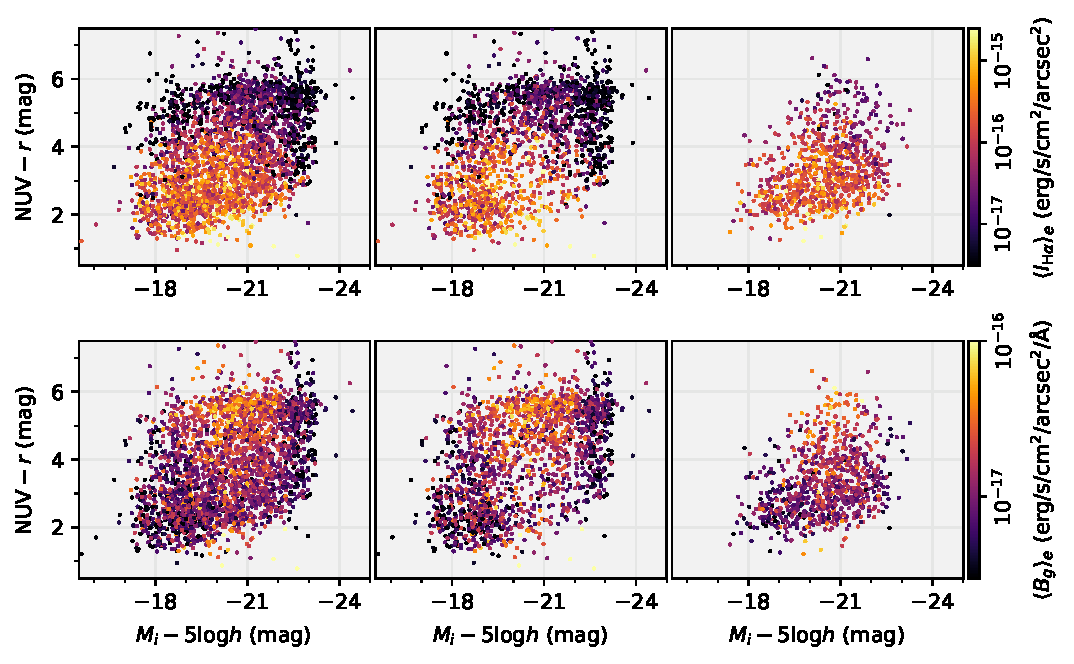
\includegraphics[width=0.8\textwidth]{figs/cmd_flux.pdf}
%
\end{center}
%
\caption{
%
${\rm N} - r$ color and absolute $i$-band magnitude ($M_i$) for all
galaxies observed during the first two years of the MaNGA Survey (left),
the subsample of galaxies {\em not} selected to be kinematically regular
(middle; see text), and the asymmetric-drift sample used throughout the
remainder of our analysis.  The color of the data points in the top row
represent the mean H$\alpha$ surface brightness [[check aperture]]
according to the colorbar to the right; the bottom row replaces the
color by the $r$-band surface brightness density.
%
}
%
\label{fig:sample}
%
\end{figure*}
%%%%%%%%%%%%%%%%%%%%%%%%%%%%%%%%%%%%%%%%%%%%%%%%%%%%%%%%%%%%%%%%%%%%%%%%

In addition to the basic understanding of this dynamically relevant
quantity, our interest in asymmetric drift stems from its fundamental
dynamical connection to the full phase-space distribution function of a
galaxy's stars, as empirically demonstrated in the Milky Way.  Indeed,
Westfall et al. (2011) (see also refs) used asymmetric drift to
constrain the axial ratios of the SVE given direct measurements of the
line-of-sight (LOS) stellar velocity dispersion, $\sigma$.
Alternatively, if one can statistically constrain the shape of the SVE
(refs), measurements of asymmetric drift could be used as a proxy for
stellar $\sigma$ by either appealing to equation \ref{eq:adformal} or an
empirical relation calibrated by samples with both asymmetric drift and
$\sigma$ measurements.  Such a use of asymmetric drift as a proxy for
stellar $\sigma$ is attractive in the low-surface-brightness and
low-velocity-dispersion regimes where direct measurements are difficult
and/or expensive.  We commit to this paradigm by using the following
nomenclature for asymmetric drift, following from equation
\ref{eq:adformal}:
%
\begin{equation}
%
\sigma_a^2 \equiv v_c^2 - \overline{v_\theta}^2.
%
\label{eq:addef}
%
\end{equation}

For disk galaxies, there is a decades-long industry of using cold-gas
tracers to construct circular-speed curves of galaxies (refs).  These
data have provided the first concrete arguments for the presence of
massive dark-matter halos (ref) based on mass model reconstruction
(refs) and have formed the basis for the most robust Tully-Fisher
relations compiled for the local Universe (refs).  However, it is
important to acknowledge that one cannot directly measure $v_c$,
effectively making $\sigma_a$ unobservable.  That is, every dynamical
tracer has some non-zero dynamical pressure such that it will lag behind
the theoretically defined circular speed.  There are very clear examples
of early-type galaxies that show differential asymmetric-drift in their
molecular (e.g., CO), atomic (e.g., \ion{H}{1}), and/or ionized
(H$\alpha$) tracers relative to a robust mass model of $v_c$ (Davis et
al.) due to the different turbulent/thermal pressures intrinsic to these
tracers.  However, these signatures are much less apparent in disk
galaxies.  For example, Martinsson et al.\ show that H$\alpha$ and
\ion{H}{1} rotation curves are consistent for the DiskMass Survey within
the limits of their constraints on beam-smearing, suggesting that any
correction for the lag of either behind the circular speed should be
small.  Indeed, theoretical calculations (Dalcanton \& Stilp) suggest
that gas-pressure corrections to \ion{H}{1} rotation curves should be
largely negligible for galaxies with ${\mathcal M} > 10^x {\mathcal
M}_\odot$.  Nevertheless, we emphasize here that our measurements of
$\sigma_a$ may be better termed as a {\em differential tangential lag}
because they are based on the quadrature difference between the observed
H$\alpha$ and stellar rotation curves in our galaxy sample (Section
\ref{sec:data}).  These measurements are perfectly valid in their own
right; however, it is their interpretation in the context of the
theoretical definition of asymmetric drift that should be questioned in
some regimes, as discussed in Section \ref{sec:discussion}.

We present the data used for our analysis in the following section.  In
Section \ref{sec:results}, we demonstrate that there is a strong
correlation between the absolute $i$-band magnitude of a galaxies and
the strength of its asymmetric drift measured at half of an effective
radius (0.5 $R_{\rm eff}$).  We also illustrate the weak color
dependence in this relation.  We summarize and discuss these results in
Section \ref{sec:discussion}.

\section{Data}
\label{sec:data}

We use integral-field spectroscopy from the SDSS-IV/MaNGA (Mapping
Nearby Galaxies from APO) Survey to construct stellar and ionized-gas
velocity fields for 2715 unique galaxies, 39 of which have multiple
observations.  The kinematic measurements are provided by the MaNGA data
analysis pipeline (DAP; Westfall et al., in prep): the ionized-gas
kinematics are based on simple single-Gaussian fits to the H$\alpha$
emission feature and the stellar kinematics are determined using pPXF
(Cappellari et al.) with the MILES stellar template library (Jesus FB et
al.).

The MaNGA galaxy selection (Wake et al. in prep) is a simple cut in
absolute $i$-band magnitude, $M_i$, and redshift, $z$, and provides a
complete sampling of the overall galaxy population.  As such,
measurements of stellar and/or H$\alpha$ rotation curves for some
systems will be difficult/impossible.  Using the photometry from the
NASA-Sloan Atlas (ref),\footnote{\url{nsatlas.org}} Figure
\ref{fig:sample} shows the color-magnitude diagram of all galaxies
colored by their mean H$\alpha$ and $r$-band surface brightness.
[[TODO: Need to check this plot.]] Although not excluded from our
velocity-field analysis {\em a priori}, we expect to obtain poor
rotation curve measurements for galaxies with low H$\alpha$ and stellar
surface brightness.\footnote{
%
The uniformity of the MaNGA survey (Law et al. 2015) is such that S/N is
tightly correlated with surface brightness.}

[[Extinction corrections for the CMD?]]

We model the geometric projection of the rotational plane of each galaxy
using the approach presented by Andersen \& Bershady (2013); see also
Westfall et al. (2011).  In three independent fitting iterations, the
model fits are optimized for the H$\alpha$ velocity field, the stellar
velocity field, and simultaneously for both data sets; for the latter,
the geometry is forced to be the same for the two dynamical tracers, but
the parametrized rotation curves are independent.  We use these
velocity-field-fitting results to objectively isolate a set of
``kinematically regular'' galaxies.  Briefly, galaxies in this sample
must have: (i) successful velocity-field fits for all three approaches,
(ii) differences in the measured H$\alpha$ and stellar systemic velocity
of less than 20 km/s, (iii) dynamical centers that are consistent to
within a fiber diameter of the morphological center [[check]], (iv)
H$\alpha$ and stellar velocity-field position angles that are consistent
to within $\pm$15$\arcdeg$, and (v) kinematic inclinations between
$15\arcdeg < i < 80\arcdeg$ that are both consistent between the
H$\alpha$ and stellar data and with respect to the photometric
ellipticity to within $\pm$20$\arcdeg$.  The constraint on the
inclination is by far the most stringent. [[give number of galaxies cut
by each criterion?]]  Applying these constraints yields a sample of 798
observations (for 790 unique galaxies) out of the 2764 observations
analyzed.  Eleven galaxies with repeat observations satisfy the
selection criteria; however, only five of these show all observations
are consistently selected, whereas the other six show one or more of the
observations did not pass our constraints [[we should understand
this.]].  [[TBD: Finally, we also visually inspected the broad-band
imaging of these 790 galaxies and eliminated merging and highly
extincted (highly inclined) systems yielding a final sample of XXX
galaxies.]]  We hereafter refer to galaxies that satisfy our selection
criteria as the ``asymmetric-drift'' sample.

Figure \ref{fig:sample} shows the color-magnitude distribution for all
MaNGA galaxies, as well as the distributions of those galaxies included
and excluded from our asymmetric-drift sample.  As expected, galaxies
with relatively high H$\alpha$ and $r$-band surface brightness are
preferentially selected, excluding much of the red sequence as well as
the brightest and faintest galaxies in the blue cloud.  Although the
conclusions we reach based on our asymmetric drift sample are
astrophysically meaningful, it is important to appreciate the biased
representation of the overall galaxy population represented by the
sample in our analysis.  [[Show histogram of kinematically regular
sample against the volume-corrected distribution of the MaNGA parent
sample in Mi and N-r, and discuss.]]

Our velocity-fitting method provides a model rotation curve fit to both
the H$\alpha$ and stellar data, each parametrized as a hyperbolic
tangent function: $v_{\rm rot} = v_{\rm flat} \tanh(R/h_v)$.  However,
our primary result is based on the error-weighted mean of the
deprojected rotation curve measurements for each dynamical tracer within
$\pm$30$\arcdeg$ of the major axis and $2\farcs5$ radial bins centered
at 0.25, 0.5, 0.75, 1.0, and 1.25 $R_{\rm eff}$ --- $R_{\rm eff}$ is the
effective radius using the elliptical Petrosian analysis from the
NASA-Sloan Atlas. [[Check that $R_{\rm eff}$ includes the multiplicative
offset to match these Petrosian and Sersic $R_{\rm eff}$ in the mean.]]
Specifically, we calculate the error-weighted mean and standard
deviation of $v_j = V_j/\cos\theta_j/\sin i$ and
%
\begin{equation}
%
\sigma_{a,j}^2 = (V_{{\rm H}\alpha,j}^2 - V_{\ast,j}^2) (\cos\theta_j
\sin i)^{-2},
%
\label{eq:dproj}
%
\end{equation}
%
where $V_j$ is the LOS measurement of each component in spaxel $j$
located at the in-plane polar coordinates $R_j$ and $\theta_j$ and $i$
is the disk inclination.

[[An example demonstrating the details of our measurements is
illustrated in Figure X.]]

We calculate errors in $v_{{\rm H}\alpha}$ and $\sigma_a$ as the
quadrature sum of the error-weighted standard error (i.e., the
error-weighted standard deviation divided by $\sqrt N$) and the
propagated error in the error-weighted mean. [[Can revisit this.
Details of error calculation not all that important.  We're dominated by
intrinsic deviations from the regression.]]

\section{Results}
\label{sec:results}

\begin{figure}
%
\begin{center}
%
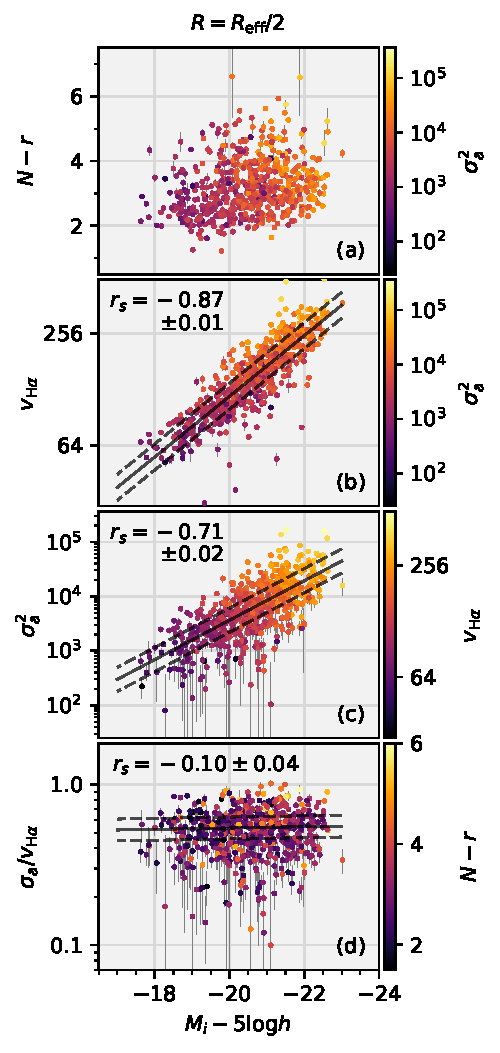
\includegraphics[width=1.0\columnwidth]{figs/mi_models.pdf}
%
\end{center}
%
\caption{
%
Global photometry measurements versus kinematics measurements at
$R=R_{\rm eff}$ for the asymmetric-drift sample: $M_i$ versus (a) $N-r$
color with each point colored according to $\sigma_a^2$, (b) $v_{{\rm
H}\alpha}$ with each point colored according to $\sigma_a^2$, (c)
$\sigma_a^2$ with each point colored according to $v_{{\rm H}\alpha}$,
and (d) $\sigma_a/v_{{\rm H}\alpha}$ with each point colored by the
$N-r$ color.  Panels (b), (c), and (d) include the Spearman rank
correlation coefficient, $r_s$, and the linear regressions (solid lines)
constructed from the median parameters provided in Table
\ref{tab:lines}.  The dashed lines are offset from linear regression by
the modeled intrinsic scatter in the relation ($\varepsilon_y$).
%
}
%
\label{fig:correlation}
%
\end{figure}

Figure \ref{fig:correlation}(a) shows the $(M_i, N-r)$ color-magnitude
diagram (see right column of Figure \ref{fig:sample}) with the points
colored according to $\sigma_a$ measured at $R=0.5R_{\rm eff}$.  There
is a clear trend where brighter galaxies have larger $\sigma_a$; the
remainder of the Figure examines this trend.

We plot $M_i$ versus $v_{{\rm H}\alpha}$, $\sigma_a^2$, and
$\sigma_a/v_{{\rm H}\alpha}$ in Figures \ref{fig:correlation}(b),
\ref{fig:correlation}(c), and \ref{fig:correlation}(d), respectively.
The points are colored according to the color bar and quantity to the
right of each panel.  Each panel provides the Spearman rank correlation
coefficient, $r_s$, of the plotted data with errors derived from $10^3$
bootstrap simulations.  We have also used a Markov Chain Monte Carlo
(refs) to sample the Bayesian posterior distribution for a linear
regression to the data in each panel, incorporating the errors in both
axes (refs); the errors in the kinematic quantities are always dominant.
The fitted model is a line in parametric form with an intrinsic Gaussian
scatter perpendicular to the line.  That is, the line is defined as
$\mathbf{l}(t) = \mathbf{l}_0 + t\ \hat{\mathbf{l}}$ for a generalized
coordinate $t$ along the line, an origin $\mathbf{l}_0 = \{x_0, y_0\}$,
and the unit vector $\hat{\mathbf{l}} = \{\cos\phi, \sin\phi\}$.  The
fitted parameters are $y_0$, $\phi$, and the dispersion of the intrinsic
Gaussian scatter about the line, $\varepsilon$; $x_0$ is fixed at the
median abscissa of the data being fitted ($x_0 = M_{i,0} = -20.6$).
Uniform priors are used for $y_0$ and $\phi$ and a logarithmic prior
[[check]] is used for $\varepsilon$ (ref).  Using the returned samples
of the posterior, we also provide parameters for the slope-intercept
form of the line --- $y = mx + b$ where $m = \tan\phi$ and $b = y_0 -
x_0 \tan\phi$ --- and the scatter projected along the ordinate,
$\varepsilon_y = \varepsilon/|\cos\phi$|.  Table \ref{tab:lines}
provides the median and standard deviation of the marginalized
distribution of each parameter; these parameters have been used to
construct the lines provided in Figure \ref{fig:correlation}.

%%%%%%%%%%%%%%%%%%%%%%%%%%%%%%%%%%%%%%%%%%%%%%%%%%%%%%%%%%%%%%%%%%%%%%%%
\begin{deluxetable}{ c r r r }
\tabletypesize{\small}
\tablewidth{0pt}
\tablecaption{Linear Regressions for $M_i$
    [[Check slope-intercept form]]}
\tablehead{ & \multicolumn{3}{c}{Dependent Variable} \\
    \cline{2-4} \\[-3pt]
 \colhead{Parameter} & \colhead{$v_{{\rm H}\alpha}$} &
 \colhead{$\log(\sigma_a^2)$} &
 \colhead{$\log(\sigma_a/v_{{\rm H}\alpha})$} }
\startdata
          $y_0$ &      2.168 &       3.78 &     -0.269 \\
                & $\pm$0.003 &  $\pm$0.01 & $\pm$0.003 \\[2pt]
         $\phi$ &     170.70 &      160.1 &      -0.24 \\
                &  $\pm$0.15 &   $\pm$0.5 &  $\pm$0.17 \\[2pt]
  $\varepsilon$ &      0.069 &      0.209 &      0.068 \\
                & $\pm$0.001 & $\pm$0.005 & $\pm$0.002 \\[2pt] \hline \\[-4pt]
            $m$ &     -0.164 &     -0.362 &     -0.004 \\
                & $\pm$0.003 & $\pm$0.009 & $\pm$0.003 \\[2pt]
            $b$ &      -1.20 &      -3.69 &      -0.36 \\
                &  $\pm$0.05 &  $\pm$0.19 &  $\pm$0.06 \\[2pt]
$\varepsilon_y$ &      0.070 &      0.222 &      0.068 \\
                & $\pm$0.001 & $\pm$0.005 & $\pm$0.002
\enddata
\label{tab:lines}
\end{deluxetable}
%%%%%%%%%%%%%%%%%%%%%%%%%%%%%%%%%%%%%%%%%%%%%%%%%%%%%%%%%%%%%%%%%%%%%%%%

As expected, there is a strong correlation between $v_{{\rm H}\alpha}$
and $M_i$.  However, it is important to note that Figure
\ref{fig:correlation}(b) does not present the Tully-Fisher (ref)
relation for our asymmetric-drift sample; the Figure gives the rotation
speed at $R=0.5R_{\rm eff}$, not a measure of the full-width of the
dynamically broadened line profile.  The slope of the relation in Figure
\ref{fig:correlation}(b) is steeper than a nominal Tully-Fisher relation
because galaxies at low luminosity tend to have more slowly rising
rotation curves (refs), which can be confirmed by plotting $h_{v,{\rm
H}\alpha}/R_{\rm eff}$ as a function of $M_i$. [[actually show this?]]

Figure \ref{fig:correlation}(c) gives the direct representation of the
gradient in the point color seen in Figure \ref{fig:correlation}(a).
The data in this panel are highly correlated, both as determined by
$r_s$ and the fitted regression.  The intrinsic scatter increases from
0.07 dex (17\%) in $(M_i,v_{{\rm H}\alpha})$ to 0.21 dex (62\%) in
$(M_i,\sigma_a^2)$; however, this is close to the $\sim$0.1 dex scatter
if considering $(M_i,\sigma_a)$ instead.

If $\sigma_a$ or $v_{{\rm H}\alpha}$ was a secondary parameter in the
distribution of $(M_i,v_{{\rm H}\alpha})$ or $(M_i,\sigma_a^2)$,
respectively, we should expect a gradient in the point color in Figures
\ref{fig:correlation}(b) and \ref{fig:correlation}(c) {\em
perpendicular} to the fitted regression.  However, we see that the
primary gradient in point color is parallel to the fitted regression.
This is consistent with the result that there is little to no
correlation between $M_i$ and $\sigma_a/v_{{\rm H}\alpha}$, as shown in
Figure \ref{fig:correlation}(d):  Both $r_s$ and $\phi$ are small and
only marginally significant with respect to their errors.  From equation
\ref{eq:dproj}, this implies that the deprojected stellar rotation is a
roughly constant fraction of the ionized-gas rotation speed, with
$v_{\ast} \sim 0.9 v_{{\rm H}\alpha}$.  Although the radius at which the
asymmetric drift was sampled is different, this ratio is consistent with
galaxies from the DiskMass survey (Martinsson et al.).

The points in Figure \ref{fig:correlation}(d) are colored by the global
$N-r$ color; however, it is difficult to determine from this
illustration if their is any correlation between $\sigma_a/v_{{\rm
H}\alpha}$ and global galaxy color.  One might expect such a correlation
if, for example, galaxies with different global color different
light-weightings of the thin vs. thick-disk (refs [[not sure there are
relevant ones]]), which propagates to a different dominant dynamical
pressure in the disk midplane.  Figure \ref{fig:colortrend} assess this
directly by plotting the error-weighted mean trend in $\sigma_a/v_{{\rm
H}\alpha}$ for the quartiles of the $N-r$ distribution of the
asymmetric-drift sample.  The error bars represent the error-weighted
standard deviation of the data in each bin, whereas the error-weighted
standard error is always smaller than the plotted point.  There is a
marginal detection of a slightly larger $\sigma_a/v_{{\rm H}\alpha}$ in
the reddest bin; however, more data would be required to lend this
result any statistical significance.

%%%%%%%%%%%%%%%%%%%%%%%%%%%%%%%%%%%%%%%%%%%%%%%%%%%%%%%%%%%%%%%%%%%%%%%%
\begin{figure}
%
\begin{center}
%
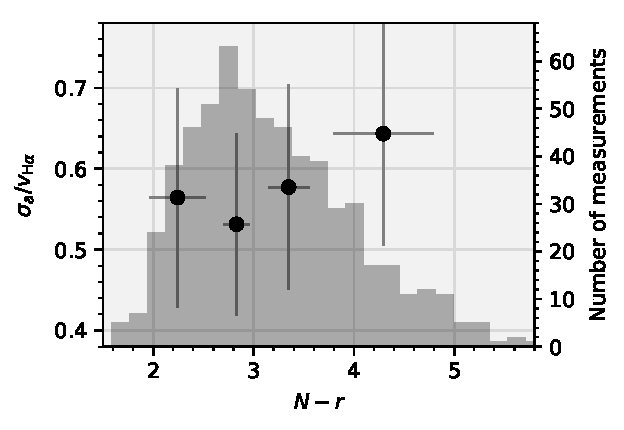
\includegraphics[width=1.0\columnwidth]{figs/adov_vs_color.pdf}
%
\end{center}
%
\caption{
%
The error-weighted mean trend in $\sigma_a/v_{{\rm H}\alpha}$ binned in
quartiles of the global $N-r$ color (black points).  The error bars
represent the error-weighted standard deviation of the data within each
bin; the error-weighted standard error is smaller than the size of each
black point.  The underlying gray histogram provides the number of
measurements in bins of $N-r$; each quartile contains $\sim$152
galaxies.
%
}
%
\label{fig:colortrend}
%
\end{figure}
%%%%%%%%%%%%%%%%%%%%%%%%%%%%%%%%%%%%%%%%%%%%%%%%%%%%%%%%%%%%%%%%%%%%%%%%

\section{Discussion}
\label{sec:discussion}

\subsection{Technical Concerns}

[[Sample bias]]

[[Beam-smearing]]

\subsection{Prospects}

If $\sigma_a$ is a direct proxy for $\sigma_R$ ...

\bibliography{master}

\end{document}


% Under the nominal assumptions of (i) a radially independent rotation
% speed and SVE shape and (ii) a exponential dispersion profile with an
% e-folding length of twice the disk scale length ($h_R$, ref), equation
% \ref{eq:adformal} can be used to show asymmetric drift will be maximum
% at 1.25$h_R$, or approximately 0.7$R_{\rm eff}$.



%\begin{deluxetable*}{ r r r r r r r r }
%\tabletypesize{\small}
%\tablewidth{0pt}
%\tablecaption{Linear Regressions for $M_i$ [[Check slope-intercept form]]}
%\tablehead{ \colhead{Dependent} & \multicolumn{3}{c}{Parametric Form} && \multicolumn{3}{c}{Slope-intercept Form} \\
%    \cline{2-4} \cline{6-8}
%    \colhead{Variable} & \colhead{$y_0$} & \colhead{$\phi$} & \colhead{$\varepsilon$} 
%                        && \colhead{$m$} & \colhead{$b$} & \colhead{$\varepsilon_y$} }
%\startdata
% $v_{{\rm H}\alpha}$                &      2.168 &    170.70 &      0.069 &&     -0.164 &     -1.20 &      0.070 \\
%                                    & $\pm$0.003 & $\pm$0.15 & $\pm$0.001 && $\pm$0.003 & $\pm$0.05 & $\pm$0.001 \\[2pt]
% $\log(\sigma_a^2)$                 &       3.78 &     160.1 &      0.209 &&     -0.362 &     -3.69 &      0.222 \\
%                                    &  $\pm$0.01 &  $\pm$0.5 & $\pm$0.005 && $\pm$0.009 & $\pm$0.19 & $\pm$0.005 \\[2pt]
% $\log(\sigma_a/v_{{\rm H}\alpha})$ &     -0.269 &     -0.24 &      0.068 &&     -0.004 &     -0.36 &      0.068 \\
%                                    & $\pm$0.003 & $\pm$0.17 & $\pm$0.002 && $\pm$0.003 & $\pm$0.06 & $\pm$0.002
%\enddata
%\label{tab:lines}
%\end{deluxetable*}


